\documentclass{article}
\usepackage[utf8]{inputenc}
\usepackage{array,multirow,graphicx}
\usepackage{amsmath,amssymb,latexsym}
\usepackage{mathabx}
\usepackage{parskip}
\usepackage{listings}
\usepackage[section]{placeins}
\usepackage{hyperref}
\usepackage[english]{babel}
\usepackage{biblatex}
\renewcommand{\sfdefault}{ptm}
\graphicspath{ {/} }

\title{Report.8.Sakila}
\author{Linh Duong}
\date{November 2017}

\begin{document}

\maketitle

\section{List names of all the languages in the database (sorted alphabetically)?}
\begin{lstlisting}[language=sql]
select name from language
order by name;
\end{lstlisting}
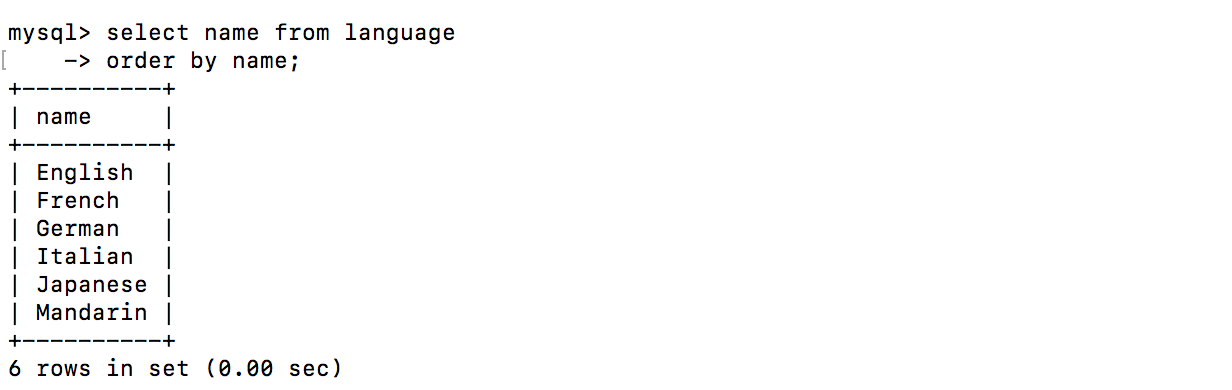
\includegraphics[width=\linewidth]{1.png}

\section{List full names of actors with "GER" in their last name, ordered by their first name}
\begin{lstlisting}[language=sql]
select concat(first_name,' ',last_name) as fullname 
from actor where last_name like '%GER%'
order by first_name;
\end{lstlisting}
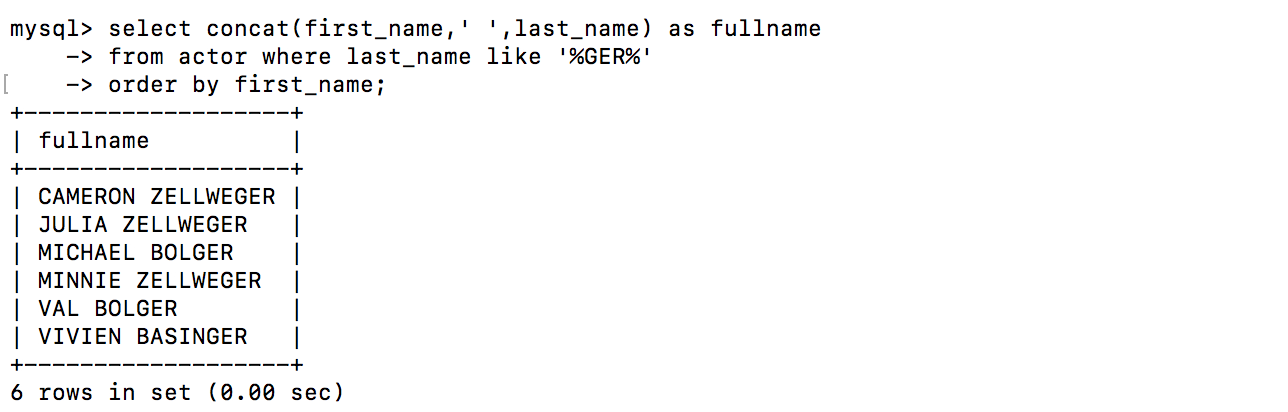
\includegraphics[width=\linewidth]{2.png}

\section{Find all the addresses where postal code starts with "57", and return addresses sorted.}
\begin{lstlisting}[language=sql]
select address from address
where postal_code like '57%'
order by address;
\end{lstlisting}
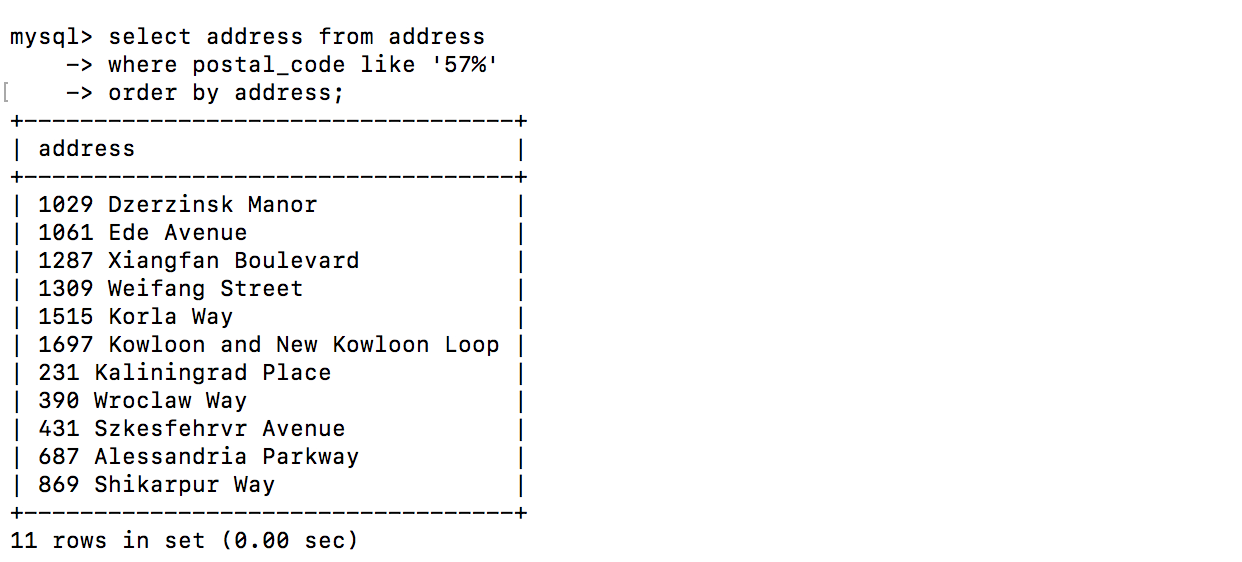
\includegraphics[width=\linewidth]{3.png}

\section{How many films involve a "DWARF" in their titles?}
\begin{lstlisting}[language=sql]
select count(title) from film_list 
where title like '%DWARF%';
\end{lstlisting}
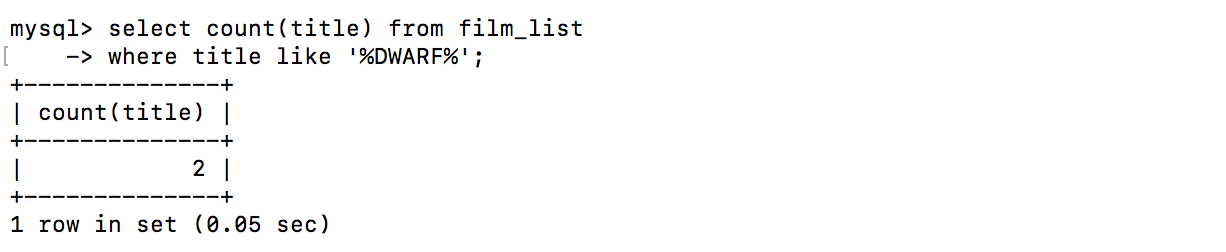
\includegraphics[width=\linewidth]{4.png}

\section{Find full names of actors who played in a film involving ’WAR’ in title and longer than 2.5 hours, along with the title, run length and release year of the movie, sorted by the actors’ last names.}
\begin{lstlisting}[language=sql]
select actors, film_list.title, film_list.length, release_year
from film_list join film on FID = film_id
where film_list.title like '%WAR%' and film.length > 150;
\end{lstlisting}
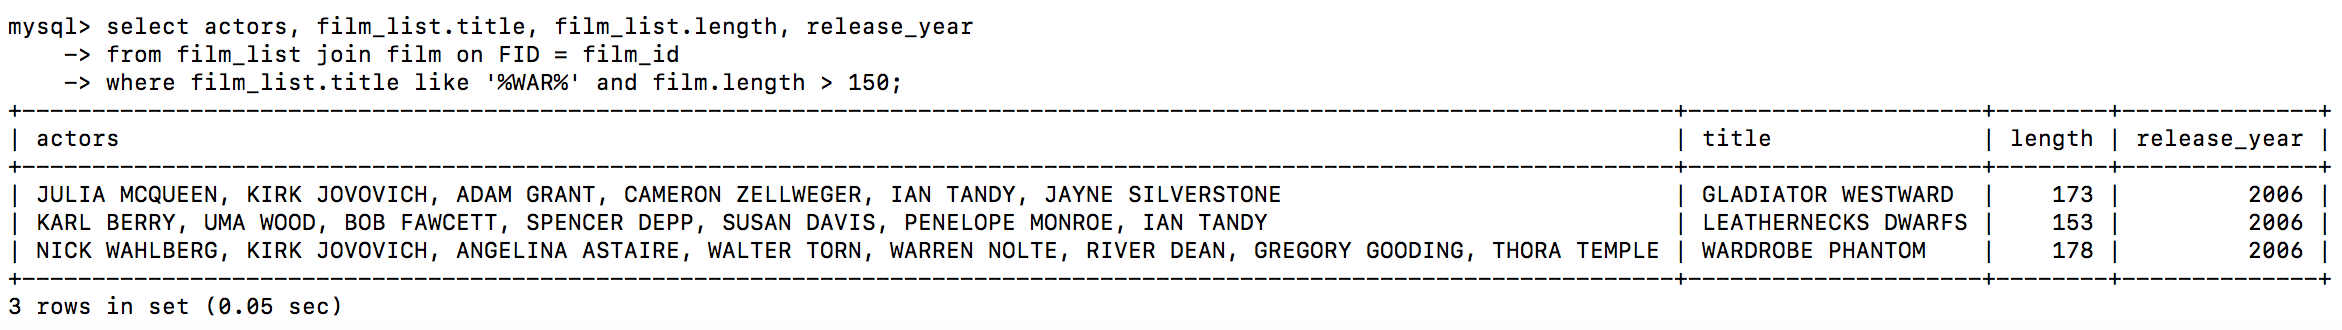
\includegraphics[width=\linewidth]{5.png}

\section{Find all the film categories in which there are between 55 and 65 films. Return the names of these categories and the number of films per category, sorted by the number of films descending}
\begin{lstlisting}[language=sql]

select name, count(film_id) as numberoffilms
from film_category 
join category on film_category.category_id=category.category_id
group by film_category.category_id 
having numberoffilms >=55 and numberoffilms <=65 ;
\end{lstlisting}
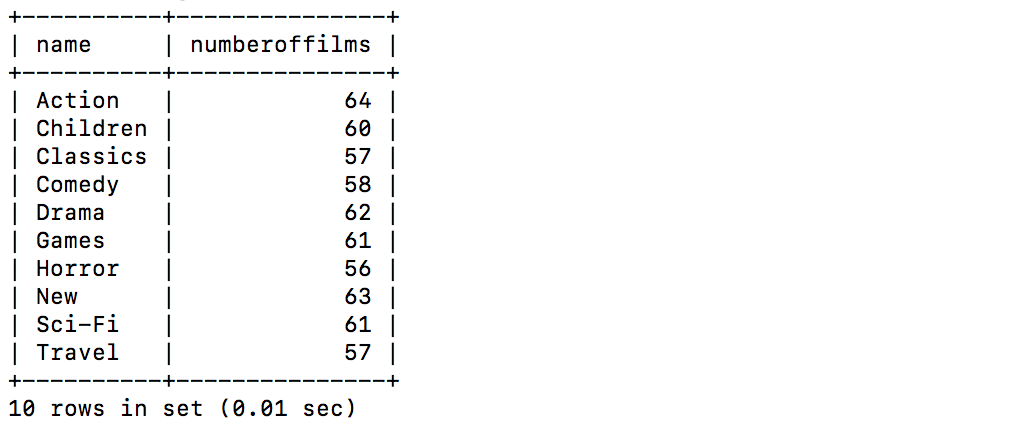
\includegraphics[width=\linewidth]{6.png}


\section{In how many film categories is the average di erence between the film replacement cost and the rental rate larger than 17?}
\begin{lstlisting}[language=sql]
select count(*) as result
from (
select category_id
from film_category
join film on film_category.film_id = film.film_id
group by film_category.category_id
having abs(avg(replacement_cost) - avg(rental_rate)) >17) as nocate;

\end{lstlisting}
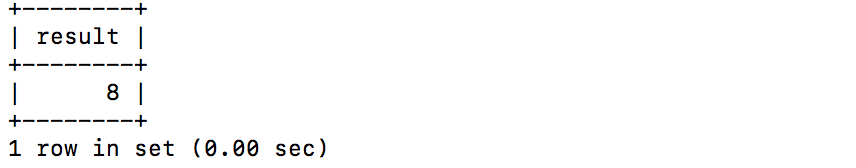
\includegraphics[width=\linewidth]{7.png}

\section{Find the address district(s) name(s) such that the minimal postal code in the district(s) is maximal over all the districts. Make sure your query ignores empty postal codes and district names.}
\begin{lstlisting}[language=sql]
select district, mincode
from 
(select district, min(postal_code) as mincode
from address
where postal_code is not null
group by district) as result
group by district
order by mincode desc limit 0,1;
\end{lstlisting}
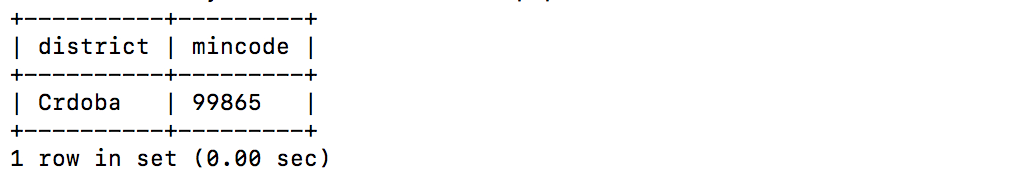
\includegraphics[width=\linewidth]{8.png}

\section{Find the names (first and last) of all the actors and customers whose first name is the same as the first name of the actor with ID 101 (exclude the actor with ID 101).}
\begin{lstlisting}[language=sql]
create view condi as 
	select first_name from actor where actor_id = 101;

select concat(first_name,' ',last_name) as fullname
from actor 
where first_name = (select * from condi)
and actor_id != 101
union 
select concat(first_name,' ',last_name) as fullname
from customer
where first_name = (select * from condi);
\end{lstlisting}
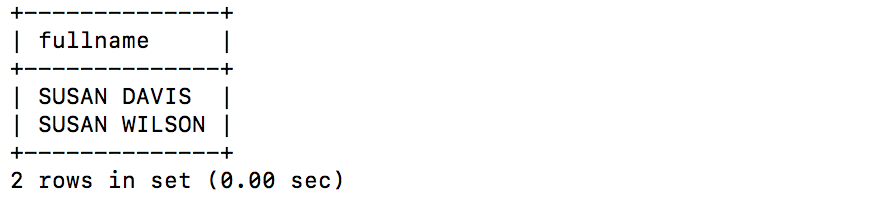
\includegraphics[width=\linewidth]{9.png}




\end{document}
